\documentclass[aspectratio=169]{beamer}
\usetheme{Madrid}
\usepackage[utf8]{inputenc}
\usepackage[T1]{fontenc}
\usepackage{tikz}
\usepackage{amssymb}
\usepackage{graphicx}
\setbeamertemplate{navigation symbols}{}
\setbeamercolor{title}{fg=white,bg=green!60!teal}
\setbeamercolor{frametitle}{fg=white,bg=green!60!teal}
\setbeamercolor{block title}{bg=green!60!teal!20,fg=black}
\setbeamercolor{block body}{bg=green!60!teal!8,fg=black}
\setbeamercolor{item}{fg=green!60!teal}
\setbeamercolor{itemize item}{fg=green!60!teal}
\setbeamertemplate{itemize item}[triangle]

\title{Read \& Report}
\subtitle{A brand new mission type --- no battle, just real data}
\author{ByteForge --- Grade 9 --- The Deep Diver}
\date{}

\begin{document}

\begin{frame}
    \titlepage
\end{frame}

\begin{frame}{Today's Missions}
    \Large
    \begin{itemize}
        \item Cargo Count
        \item Crew Roster
    \end{itemize}
\end{frame}

\begin{frame}{A list of records, and ONE function: answer()}
    \large
    \begin{itemize}
        \item \texttt{data} is a list of records --- each has named fields like item, weight
        \item Loop through every record, add up a total, call \texttt{answer(value)} exactly once
    \end{itemize}
\end{frame}


\begin{frame}{This is an extremely common real task}
    \large
    \begin{itemize}
        \item "Loop a table, total one column" --- spreadsheets and databases do this constantly
    \end{itemize}
\end{frame}


\begin{frame}{Finding a maximum --- why it MUST be a loop}
    \large
    \begin{itemize}
        \item Cannot hardcode "the third one" --- has to work for ANY list, not just this data
        \item Assume the first record is best, check every other record
    \end{itemize}
\end{frame}

\begin{frame}{Real-World Examples}
    \large
    \begin{itemize}
        \item A school attendance spreadsheet totalling absences per student is EXACTLY this pattern --- loop, add, report.
    \end{itemize}
\end{frame}


\begin{frame}{Image}
    \begin{center}
    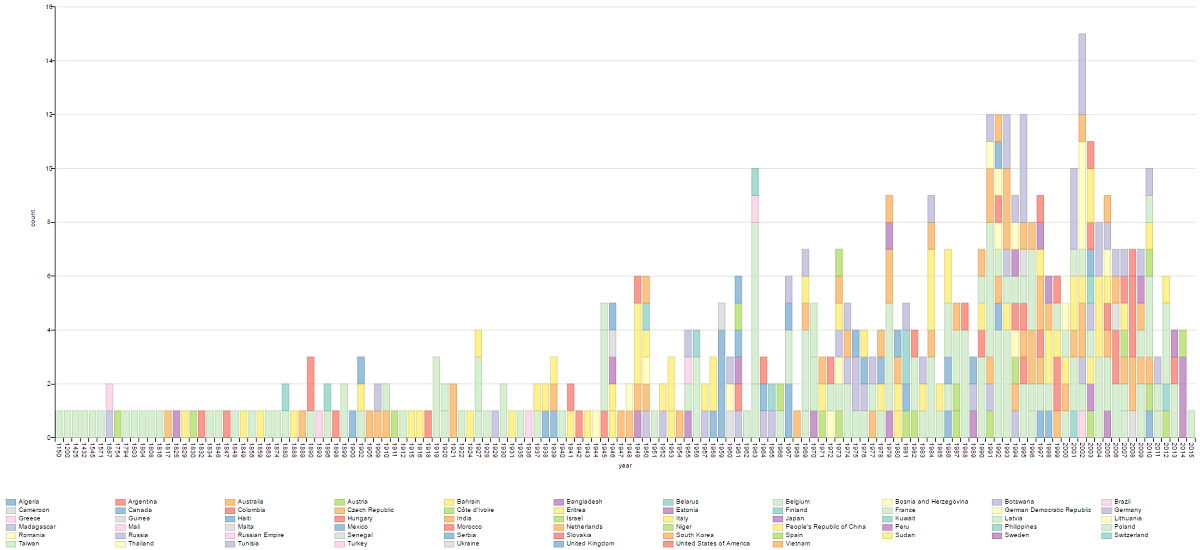
\includegraphics[width=0.5\textwidth]{images/barchart.png}

    \large Real data, visualised --- once you can total and scan a table like this chapter teaches, a real chart like this is one small step further.

    \small Bar chart --- Egorik H, public domain / CC BY-SA 4.0, via Wikimedia Commons
    \end{center}
\end{frame}

\begin{frame}{Let Them Discover}
    \large
    Given a class of 5 students' test scores, work out the total and the highest score by hand, tracking both as you go --- the same dual-tracking this chapter needs.
\end{frame}

\begin{frame}{Your Turn}
    \Large
    Open the mission map, find \textbf{Read \& Report}, and fly it for real ---
    everything you just saw, you now do yourself.
\end{frame}

\end{document}
